
\documentclass[12pt]{article}

\usepackage{graphicx}
%\usepackage{subcaption}
\usepackage{amsmath}
\usepackage{amssymb}
%\usepackage{afterpage}
%\usepackage{showlabels}
% \usepackage{epstopdf}
% \usepackage{pdfpages}
\usepackage{geometry}
%\usepackage{wrapfig}
\usepackage{url}
\usepackage{times}
\usepackage{pdfpages}
\usepackage{etoolbox}
\usepackage{hyperref}
\usepackage{enumitem}
\hypersetup{
    colorlinks=true,
    linkcolor=blue,
    filecolor=magenta,
    urlcolor=cyan,
    pdftitle={Overleaf Example},
    pdfpagemode=FullScreen,
    }

\urlstyle{same}

\newcommand{\s}{\textrm{s}}
\newcommand{\m}{\textrm{m}}
\newcommand{\kg}{\textrm{kg}}
\newcommand{\N}{\textrm{N}}
\DeclareMathOperator{\sech}{sech}
\DeclareMathOperator{\arctanh}{arctanh}

\newcommand{\shortlist}{%
\parindent 0in%
\parskip   0in%
\itemsep   0in%
\topsep    0in%
\parsep    0in%
}

\setlength{\parindent}{0in}

\geometry{letterpaper,tmargin=1in,bmargin=1in,lmargin=1in,rmargin=1in}

\newcommand{\soln}[1] {\textit{Solution:} #1}

\newcommand{\Title}{PHYS 615 -- HW 4}

\begin{document}

\begin{center}
  {\Large\bfseries\Title}

\end{center}
\bigskip
\bigskip

\textbf{Types of homework questions}
\begin{itemize}\shortlist
  \item	RQ (Reading questions):  prompt you to go back to the text and read and think about the text more carefully and explain in your own words. While not directly tested in quizzes, can help you think more deeply about quiz questions.
  \item	BF (Building foundations):  gives you an opportunity to build and practice foundational skills that you have, presumably, seen before.
  \item	TQQ (typical quiz questions):   Similar questions (though perhaps longer or shorter) will be asked on quizzes.  But the difficulty level and skills tested will be similar.
  \item Design (D):  These are questions in which you are given a desired outcome and asked to figure out how to make it happen.  These will often also be TQQ’s, but always starting with desired motion/behavior as the given.
  \item	COMP (Computing): computing questions often related to TQQ but will never be asked on a quiz (since debugging can take so long).  You will need to do at least four computing questions over the semester
  \item	FC (free choice): allows you to decide where to put your time.  Any of the following are possible:  work through a section of the text or a lecture in detail; redo a problem from before; do an unassigned problem in the text; extend a computing project; try a problem using a different analytical approach (e.g. forces instead of conservation of energy).
  \item ACT (in-class activity): These questions are repeats of questions (or similar to) that occurred in a previous in-class activity.
  \item \textbf{Standard Reading Questions}: How does the reading connect with what you already know? What was something new?  Ask an "I wonder" question OR give an example applying the idea in the reading.
\end{itemize}

\textbf{Please remember to say something about the "Check/Learn" part at the end of solving a problem!}

Note that while this homework does not have designated "RQ" questions, in particular the activity-based questions can certainly benefit from reading the corresponding sections in the text.

Full credit will be given at 75\% of the total points possible, so you can choose a subset of problems (you can do more / all, but the score is capped at 75\%)

\begin{enumerate}
  \item TQQ / ACT (25 points) Hand in Activity 2.3.

        \soln{See Activity 2.3 solution.}

  \item TQQ / ACT (25 points) Someone (not you, obviously) is trying to shoot down a balloon that's up at 60,000 feet.

        \begin{enumerate}
          \item Let's presume you have a 9mm hand gun. That is to say, the diameter of the projectile is 9 mm, and its mass is 8.5 g. Let's assume a drag coefficient of $C_D = 0.2$, and the initial speed of the bullet is $450 \m/\s$, and an air density of $1.225 \kg/\m$. Even though now I've given you all those numbers, don't plug them in until the very end!
                % FIXME, should not have been item

          \item Assuming there's no drag at all, how high can the bullet reach? (You can do this any way you want, whatever seems most convenient.)

                \soln{Conservation of energy is pretty convenient, since in the beginning the pullet has only kinetic energy $\frac{1}{2}mv^2$, and at the peak, only gravitational potential energy $mgh$:
                  $$
                    \frac{1}{2}mv^2 = mgh \qquad \Longrightarrow \qquad h = \frac{v^2}{2g} \approx 20,600\,\m
                  $$
                  That actually is about 60,000 ft (spy balloon altitude).
                }

          \item Now solve the problem with drag $F_D = \frac{1}{2} \rho A C_D v^2$, where $A$ is the cross section of the projectile. In order to do so, follow the steps from Activity 2.4 -- but now the projectile is moving upward.

                Some notes:
                \begin{itemize}
                  \item The ODE will be similar but not the same, as some signs change. You might want to pick the up direction to be positive.
                  \item Even though there is no terminal velocity  while moving upward, one can still define a $v_{ter}$ as before and use it to simplify the equation. (Not required, but makes it look more familiar.)
                  \item Obviously, there needs to be a non-zero initial condition for the velocity, rather than zero.
                  \item Since the ODE isn't quite the same, the guess I gave you won't work. Since the integral that comes up when solving this by separation of variables is not trivial, you might want to ask Wolfram Alpha or some integration tables for help (e.g., \url{https://en.wikipedia.org/wiki/List_of_integrals_of_rational_functions})
                  \item If the hand gun isn't good enough, you might try again with a more powerful higher caliber gun.
                \end{itemize}


                \soln{
                  \begin{enumerate}
                    \item I'm choosing the up direction to be positive. Since the bullet is moving up, both drag and gravity are down:
                          $$m\dot v = -mg - cv^2 \qquad \Longrightarrow \qquad \dot v = -g - \frac{c}{m} v^2$$

                    \item There is no terminal velocity during upward motion -- however, I can just use the same $v_{ter}$ expression to give me some kind of a "typical velocity" that I can use to simplify my expression, so I'll do that, and I'll keep the $v_{ter}$ name, even though it's kinda a misnomer now.
                          $$v_{ter} = \sqrt{\frac{mg}{c}}$$

                    \item Rewriting the equation in terms of $v_{ter}$ (by factoring out $g$):
                          \begin{align*}
                            \dot v = -g \left(1 + \left(\frac{v}{v_{ter}}\right)^2\right)
                          \end{align*}

                    \item Since I don't have a guess for the solution, I'll try to actually solve using separation of variables:
                          \begin{align*}
                            \int_{v_0}^v \frac{dv'}{1 + \left(\frac{v'}{v_{ter}}\right)^2} = -\int_0^t g\, dt'
                          \end{align*}
                          The integral on the r.h.s. is straightforward, but the l.h.s. needs work. I can make it a bit simpler by substituting $u = v'/v_{ter}$, ie., $dv' = v_{ter} du$ and then find in a table of integrals like the wikipedia one I linked:
                          \begin{align*}
                            v_{ter} \int_{v_0/v{ter}}^{v/v_{ter}} \frac{du}{1 + u^2} & = v_{ter} \left. \arctan u\right|_{v_0/v_{ter}}^{v/v_{ter}} \\
                                                                                     & = v_{ter} (\arctan v/v_{ter} - \arctan {v_0/v_{ter}})
                          \end{align*}

                          Plugging that l.h.s. back into the above and integrating the rhs, too:
                          \begin{align*}
                            v_{ter} (\arctan v/v_{ter} - \arctan v_0/v_{ter}) & = -gt                                          \\
                            \arctan v/v_{ter} - \arctan v_0/v_{ter}           & = -\frac{g}{v_{ter}}t = -t/\tau                \\
                            \arctan v/v_{ter}                                 & = -t/\tau + \arctan v_0/v_{ter}                \\
                            v                                                 & = v_{ter} \tan (-t/\tau + \arctan v_0/v_{ter}) \\
                          \end{align*}
                          where I introduced a typical time $\tau = v_{ter}/g$.

                          This doesn't look particularly enlightening, but I plotted it, together with the numerical simulation of our ODE:

                          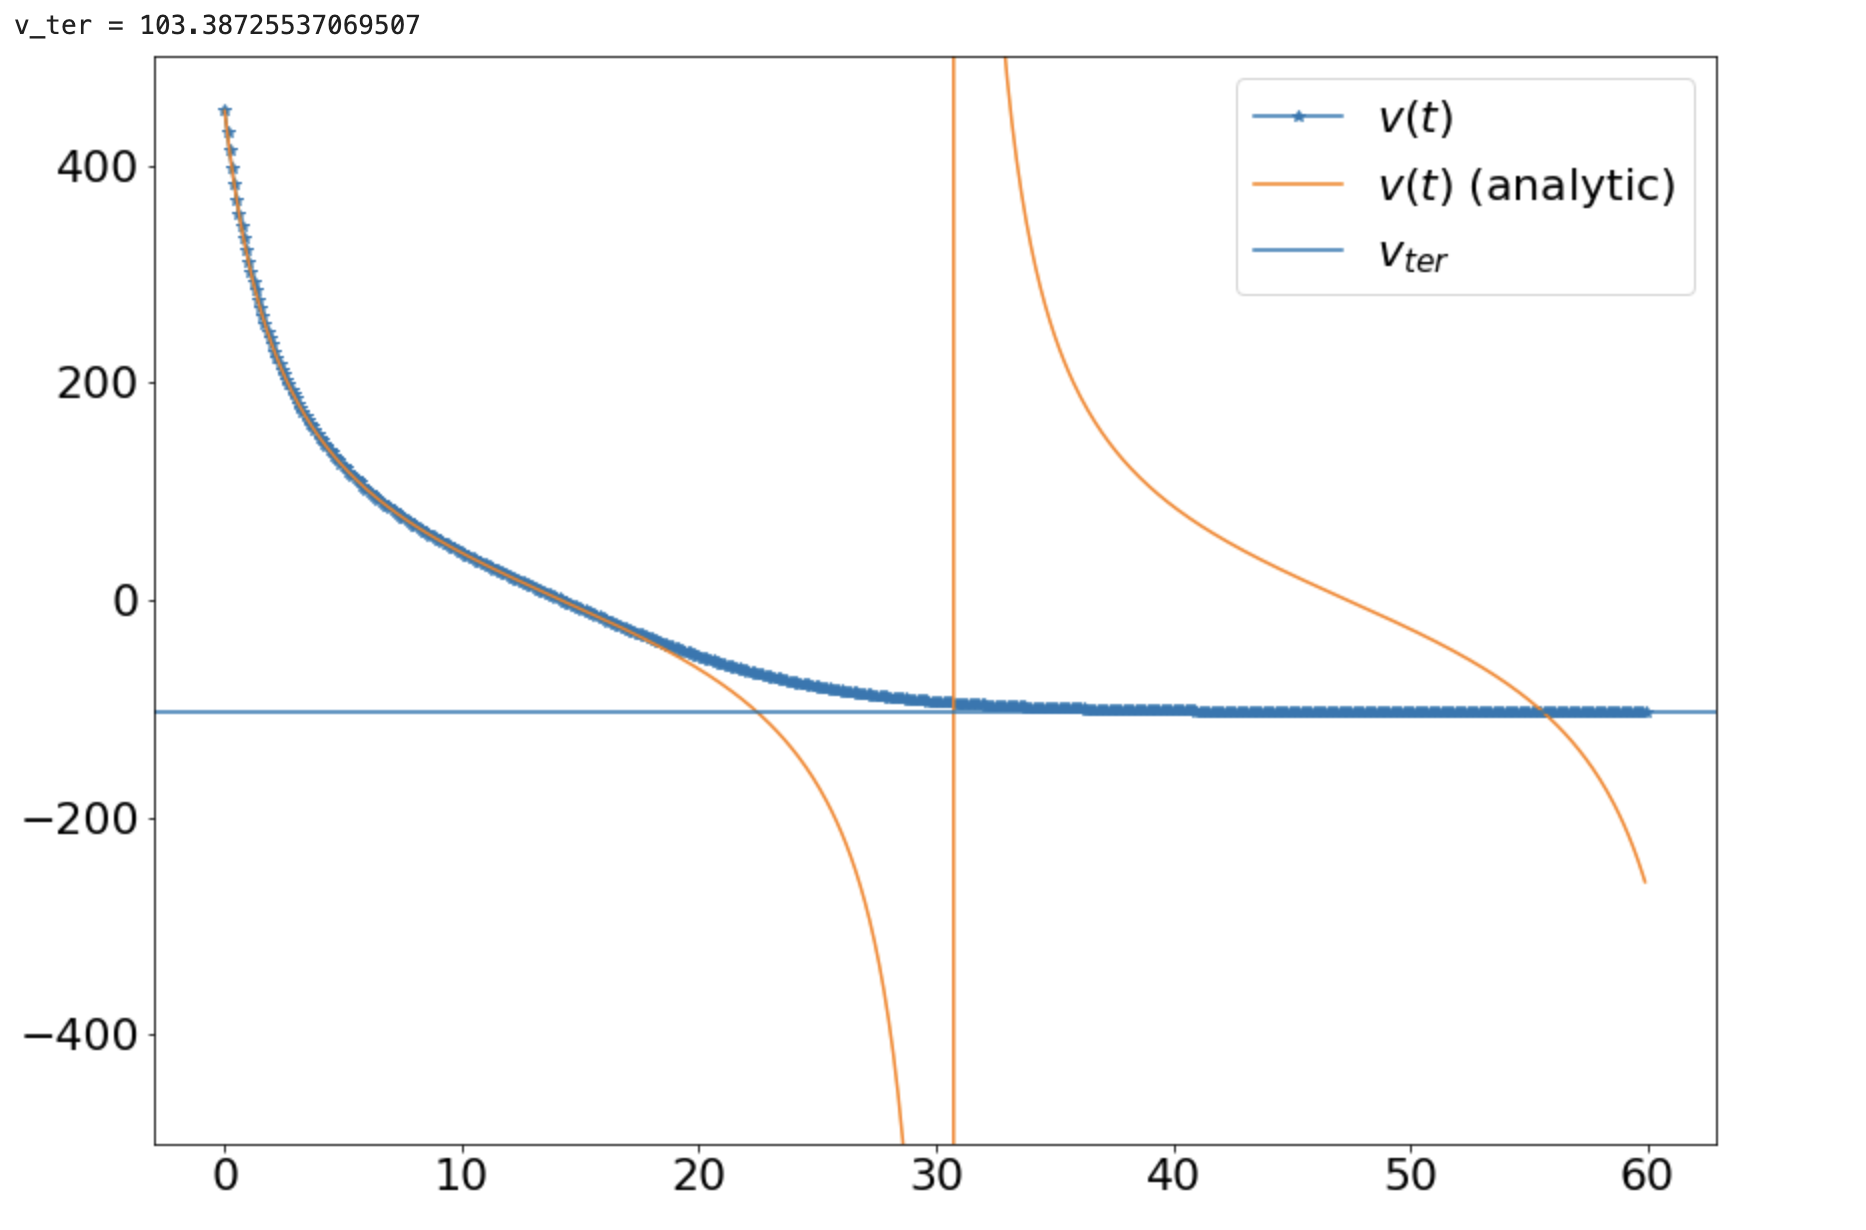
\includegraphics[width=.6\textwidth]{bullet_v.png}

                          The good news is that the analytic solution we just got matches the numerical simulation, up to the time where velocity slowed down to zero, ie., the peak. After that, velocity becomes negative, so drag should now be positive, but actually that's not the case in the ODE we're solving since we assumed velocity is up (positive). In the numerical solution, I did account for this, but our analytic solution just becomes invalid. It doesn't matter, since we're trying to find the peak height.

                    \item Well, to finally get the height, we still need to integrate one more time to get $v(t)$. I'm again using an integratal table, though this can be solved by substitution $u = \cos \ldots$.
                          \begin{align*}
                            y(t) & = \int v_{ter} \tan (-t/\tau + \arctan v_0/v_{ter})         \\
                                 & = v_{ter} \tau \ln \cos (-t/\tau + \arctan v_0/v_{ter}) + C
                          \end{align*}

                          I still need to find $C$ given by the initial condition $y(0) = 0$, so
                          $$
                            C = - v_{ter} \tau \ln \cos (\arctan v_0/v_{ter})
                          $$

                          Now I'm ready to plot this, too, to see where it matches my expectations and the numerical solution -- and again, up to the peak, it does.

                          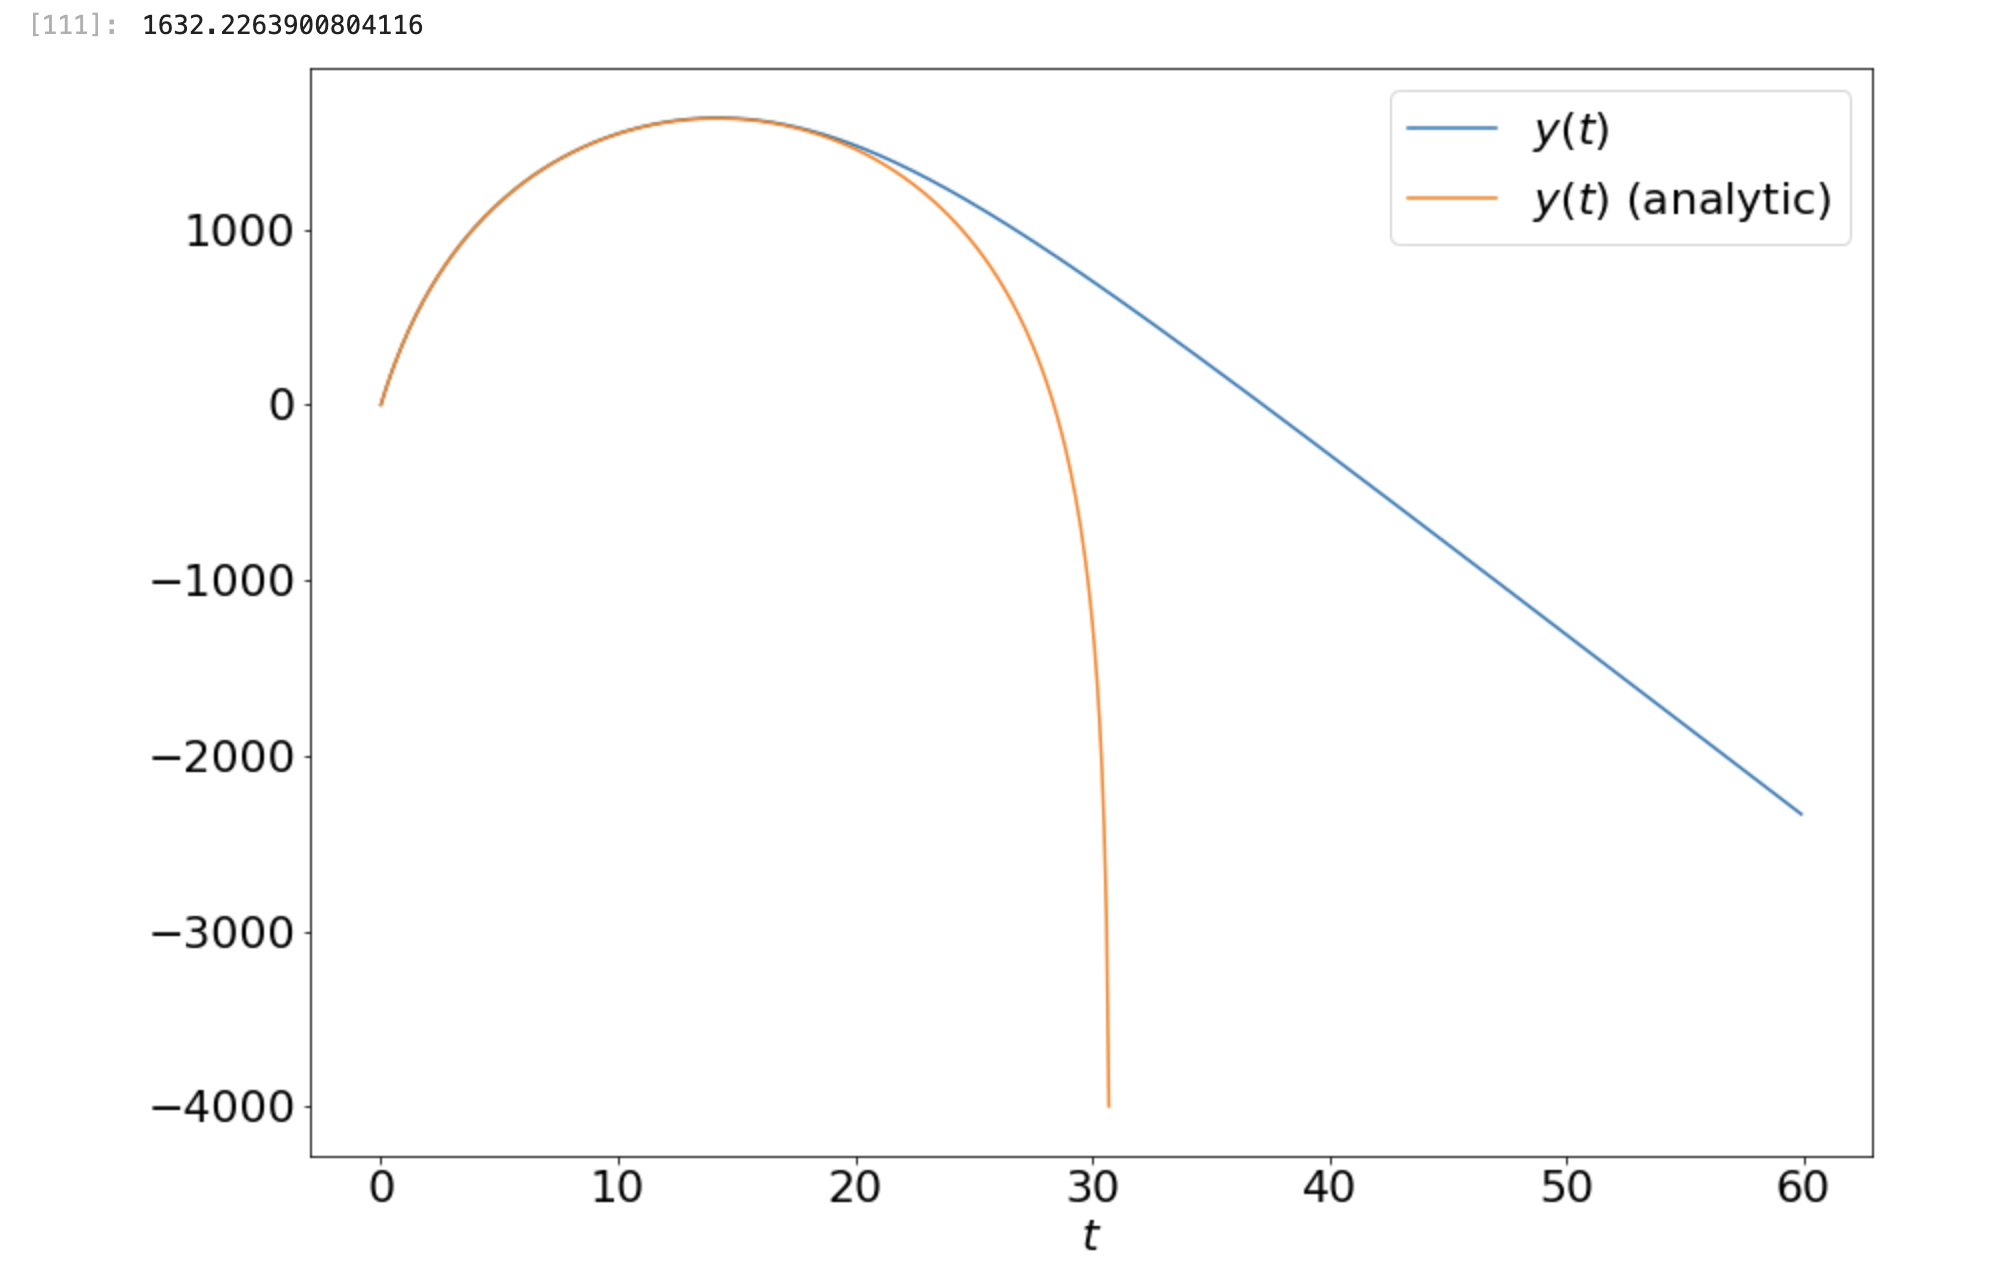
\includegraphics[width=.6\textwidth]{bullet_y.png}

                          (At later times, the valid solution becomes approximately a straight line, showing that the bullet reached terminal velocity.)

                    \item I suppose this all is kind of a demonstration that solving this numerically is much less hassle once one has the tools in place, while all the math is a bit of pain. But since we got so far, let's do the final piece, too: We need to find the time when the peak is reach to plug into $y(t)$ to get the peak height. This is not too bad, actually, since the time of the peak is when velocity is down to zero, and then tangent reaches zero when its argument does:
                          \begin{align*}
                                                   & 0                        = v(t_{peak}) = v_{ter} \tan (-t_{peak}/\tau + \arctan v_0/v_{ter}) \\
                            \Longrightarrow \qquad & t_{peak} = \tau \arctan v_0/v_{ter}
                          \end{align*}
                          Plugging this back into $y(t)$, the argument of the cosine will be zero, so the cosine is 1, and the log of 1 is zero, which leaves
                          \begin{align*}
                            y(t_{peak}) & = v_{ter} \tau \ln \cos (-t_{peak}/\tau + \arctan v_0/v_{ter}) + C \\
                                        & = C                                                                \\
                                        & = - v_{ter} \tau \ln \cos (\arctan v_0/v_{ter})
                          \end{align*}

                          Plugging in numbers, I get $y(t_{peak}) \approx 1630\,\m$, which is consistent with what the plot shows.

                          Well, while that is pretty high, it's not even close to sky balloon height...
                  \end{enumerate}

                }
        \end{enumerate}

  \item TQQ / BF (10 points) More on hyperbolic functions (see last HW for some intro)
        \begin{enumerate}
          \item Show that $\cosh z = \cos (iz)$. What is the corresponding relation for $\sinh$?

                \soln{
                  \begin{align*}
                    \cos(iz) = \frac{e^{iiz} + e^{-iiz}}{2} =
                    \frac{e^{-z} + e^{z}}{2} = \cosh z
                  \end{align*}

                  For sin/sinh, we can make the same guess:
                  \begin{align*}
                    \sin(iz) & = \frac{e^{iiz} - e^{-iiz}}{2i} =
                    \frac{e^{-z} - e^{z}}{2i}                    \\
                             & = \frac{e^{z} - e^{-z}}{-2i}      \\
                             & = \frac{1}{-i} \sinh z            \\
                             & = i \sinh z
                  \end{align*}
                  Or one can multiply the whole thing by $-i$ to get $\sinh z = -i \sin (iz)$.

                }
          \item Show that $\cosh^2 z - \sinh^2 z = 1$.

                \soln{See last homework.}

          \item What is the derivative of $\tanh z$?

                \soln{We can use the quotient rule:

                  \begin{align*}
                    \frac{d}{dz} \tanh z & = \frac{d}{dz}\frac{\sinh z}{\cosh z} = \frac{\sinh' z \cosh z - \sinh z \cosh' z}{\cosh^2 z} \\
                                         & =  \frac{\cosh^2 z - \sinh^2 z}{\cosh^2 z} = \frac{1}{\cosh^2 z} = \sech^2 z
                  \end{align*}
                }

          \item Show that $\int \tanh z \, dz = \ln\cosh z$.

                \soln{Taking the derivative of the r.h.s., remembering the chain rule:
                  $$\frac{d}{dz} \ln\cosh z = \frac{1}{\cosh z}\sinh z = \tanh z
                  $$}

          \item Prove that $1 - \tanh^2 z = \sech^2 z$, where $\sech z = 1/\cosh z$.

                \soln{
                  $$1 - \tanh^2 z = 1 - \frac{\sinh^2 z}{\cosh^2 z} = \frac{\cosh^2 - \sinh^2}{\cosh^2} =\frac{1}{\cosh^z} = \sech^2 z$$
                }
          \item Show that $\int dx / (1-x^2) = \tanh^{-1} x$. ($\tanh^{-1}$ is also called $\arctanh$.)

                \soln{Again, I'm taking the derivative of the r.h.s. The derivative of the inverse of a function is one over the derivative of the function itself:

                  \begin{align*}
                    \frac{d}{dx}  \tanh^{-1} x & = \frac{1}{\tanh' (\tanh^{-1} x)} = \cosh^2  (\tanh^{-1} x) \\
                                               & = \frac{1}{1-\tanh^2 (\tanh^{-1} x)} = \frac{1}{1-x^2}
                  \end{align*}

                }

        \end{enumerate}


  \item TQQ (5 points)

        The transverse velocity of the gyrating particle (see Taylor 2.5, 2.7) is contained in Taylor Eq. (2.77), since $\eta = v_x + i v_y$. By taking the real and imaginary parts, find expressions for $v_x$ and $v_y$ separately. Based on these expressions, describe the time dependence of the transverse velocity.

        \soln{
          Using Eq (2.77) $\eta = a e^{i(\delta - \omega t)}$, I only need to use Euler's formula:

          \begin{align*}
            v_x + i v_y & = \eta = a e^{i(\delta - \omega t)} = a \cos (\delta - \omega t) + i a \sin(\delta - \omega t)
          \end{align*}
          I can directly see that
          \begin{align*}
            v_x & = a \cos (\delta - \omega t) \\
            v_y & = a \sin (\delta - \omega t)
          \end{align*}
        }


  \item TQQ (10 points)

        In Activity 2.5 (and Taylor 2.5), we solved the motion of a gyrating particle using the trick $\eta = v_x + i v_y$. Instead, use the way that I briefly pointed out in class: Take the equation of motion for $\dot v_x$ and differentiate it one more time with respect to time. Then use the equation of motion for $\dot v_y$ to substitute into the r.h.s. You should obtain an uncoupled 2nd order ODE for $v_x$ that we have solved before (by making an educated guess, for the small angle approximation of the skateboard problem.) Use this known solution for $v_x$, and you can then find $v_y$ from your original ODEs.

        Show that the solution you obtain is equivalent to the one in Taylor Eq. (2.77).

        \soln{Here's the original system of ODEs again:

          \begin{align*}
            \dot v_x & = \omega_0 v_y   \\
            \dot v_y & = - \omega_0 v_x \\
          \end{align*}

          Differentiating the 1st equation one more time and using the 2nd equation to substitute $\dot v_y$:
          \begin{align*}
            \ddot v_x & = \omega_0 \dot v_y  = - \omega_0^2 v_x
          \end{align*}

          That is exactly the small angle skateboard equation, so we know the solution $v_x = A\cos \omega_0 t + B\sin\omega_0 t$. To find $v_y$, I use the first ODE again:
          \begin{align*}
            v_y & = \frac{1}{\omega_0} \dot v_x = \frac{A}{\omega_0} (-\omega_0 \sin \omega_0 t) + \frac{B}{\omega_0} \omega_0 \cos \omega_0 t \\
                & = -A \sin \omega_0 t + B \cos\omega_0 t
          \end{align*}

          Setting, e.g., $A = a$, $B = 0$, I have $v_x = a \cos \omega t$ and $v_y = -a \sin \omega t$, which does correspond to the solution from the previous problem with $\delta = 0$ and taking into account that $-a \sin \omega t = a \sin (-\omega t)$ and $a \cos \omega t = a \cos (-\omega t)$.
        }

  \item	FC (10 points) (free choice): allows you to decide where to put your time.  Any of the following are possible: work through a section of the text or a lecture in detail; polish up a group work assignment from class; redo a problem from before; do an unassigned problem in the text; extend a computing project; try a problem using a different analytical approach (e.g. forces instead of conservation of energy).

\end{enumerate}

\end{document}
